\section{結論及び展望}

本研究では,SE(3)上における協調自己位置推定のための視野共有を保証する分散型CBFを提案した.特に,複数のエージェントが共通の特徴点を観測することで,自己位置推定の精度を向上させるための制御手法を開発した.以下に今後の展望について述べる.

\subsection{確率関数の設計によるアクティブパーセプション}

視野共有を保証するCBFにおいては,特徴点$q_l$がエージェント$i$の視野内にあるかどうかを表す関数$\Psi_{i}^l$が重要な役割を果たす.\Eqref{eq:single_fov_condition}で示したように,この関数は以下のように定義される:
\begin{equation}
\begin{aligned}
\Psi_{i}^l = \left\{ \begin{array}{ll}
0 & \mathrm{if} \quad  \beta_l^{\top}(p_i)R_ie_c-\cos\Psi_{\mathcal{F}} < 0\\
1 & \mathrm{if}  \quad  \beta_l^{\top}(p_i)R_ie_c-\cos\Psi_{\mathcal{F}} \geq 0
\end{array} \right.
\end{aligned}
\label{eq:psi_function}
\end{equation}

しかし,この関数は微分不可能であるため,CBFの設計において問題となる.そこで本研究では,特徴点$q_l \in \mathcal{L}$によってエージェント$i$における推定が成り立っている確率を表す関数$\phi_{i}^l$を導入した:
\begin{equation}
\begin{aligned}
\phi_{i}^l= P(p_i,R_i,q^l)
\end{aligned}
\label{eq:phi_function}
\end{equation}

本研究では,簡単のために以下の確率関数を使用した:
\begin{equation}
\begin{aligned}
P_i^l &= \frac{\beta_l^\top(p_i) R_i e_c -\cos\Psi_{\mathcal{F}} }{1-\cos\Psi_{\mathcal{F}}}
\end{aligned}
\label{eq:p_function}
\end{equation}
ここで,$\beta_l$はエージェント$i$から特徴点$q_l$への単位方向ベクトル,$R_i$はエージェント$i$の姿勢行列,$e_c$はカメラの光軸方向を表す単位ベクトル,$\Psi_{\mathcal{F}}$はカメラの視野角の半分である.この確率関数は,特徴点がカメラの光軸に近いほど高い値を取り,視野角の境界では0になるという性質を持つ.

\subsection{自己位置推定における確率関数の理論的裏付け}

$P^l_i$が$(p_i, R_i)\in \mathrm{SE(3)}$について微分可能であれば,任意の確率関数を設計可能である.本研究では,自己位置推定における理論的な裏付けに基づいた確率関数の設計について検討した.

各エージェント$i \in \mathcal{A}$に対して,観測モデルは以下のように表される:
\begin{equation}
\begin{aligned}
\tilde{p}_i = \pi_i(q_l) + w_i
\end{aligned}
\label{eq:observation_model}
\end{equation}
ここで,$\pi_i(q_l)$はエージェント$i$における$q_l$の非線形な投影関数であり,$w_i$は白色ノイズである.通常,$w_i$は独立同分布の正規分布$w_i \sim \mathcal{N}(0, \sigma_i^2 I)$と仮定される.

最尤推定量$\hat{q}_l$は,以下の最適化問題の解として求められる:
\begin{equation}
\begin{aligned}
\hat{q}_l = \operatorname*{arg\,min}_{q_l} \sum_i \| \tilde{p}_i - \pi_i(q_l) \|^2_{\Sigma_i^{-1}}
\end{aligned}
\label{eq:mle}
\end{equation}
ここで,$\Sigma_i$は$w_i$の共分散行列である.

投影関数$\pi_i(q_l)$は一般に非線形であるため,解析的に誤差伝搬や不確かさを評価するには,$q_l$の推定値の周りで一階テイラー展開を用いる.任意の推定点$q_0^l$周りで:
\begin{equation}
\begin{aligned}
\pi_i(q_l) \approx \pi_i(q_0^l) + J_i (q_l - q_0^l)
\end{aligned}
\label{eq:taylor_expansion}
\end{equation}
と近似する.ここで,$J_i = \frac{\partial \pi_i}{\partial q_l} \Big|_{q_l=q_0^l}$はエージェント$i$における投影関数のヤコビアンである.

最尤推定問題において,推定値の下界としてのCramer-Rao Lower Bound (CRLB)は,フィッシャー情報行列$\mathbf{I}(q_l)$を用いて記述される:
\begin{equation}
\begin{aligned}
\mathbf{I}(q_l) = \sum_i J_i^T \Sigma_i^{-1} J_i
\end{aligned}
\label{eq:fim}
\end{equation}

\begin{dfn}[Cramer--Rao Lower Bound]
確率変数 $\mathbf y\in\mathbb R^{m}$ が母数 $\boldsymbol\theta\in\mathbb R^{p}$ に依存し,
確率密度 $p(\mathbf y;\boldsymbol\theta)$ をもつとする.  
$\hat{\boldsymbol\theta}(\mathbf y)$ が $\boldsymbol\theta$ の不偏推定量
(すなわち $\mathbb E[\hat{\boldsymbol\theta}]=\boldsymbol\theta$)であるとき,
その共分散行列は
\[
    \operatorname{Cov}(\hat{\boldsymbol\theta})
    \;\succeq\;
    \mathbf I(\boldsymbol\theta)^{-1},
    \qquad
    \mathbf I(\boldsymbol\theta)
    :=\mathbb E\!\left[
        \left(\nabla_{\!\boldsymbol\theta}\!\log p(\mathbf y;\boldsymbol\theta)\right)
        \,\left(\nabla_{\!\boldsymbol\theta}\!\log p(\mathbf y;\boldsymbol\theta)\right)^{\!\top}
    \right]
\]
で下から抑えられる.  
ここで $\mathbf I(\boldsymbol\theta)$ は
フィッシャー情報行列と呼ばれる行列である.
この不等式をCramer--Rao Lower Boundと呼ぶ.
\end{dfn}

観測モデル\eqref{eq:observation_model}の下で,パラメータ$q_l$に関する対数尤度関数を
\begin{equation}
\begin{aligned}
\ell(q_l)
&= -\frac{1}{2}\sum_{i=1}^m
(\tilde p_i - \pi_i(q_l))^\top \Sigma_i^{-1}(\tilde p_i - \pi_i(q_l)) + C
\label{eq:loglikelihood_expanded}
\end{aligned}
\end{equation}
と書く。ここで$C$は$q_l$に依存しない定数である。

まず,$\ell(q_l)$の勾配(一次微分)を計算すると
\begin{equation}
\begin{aligned}
\nabla_{q_l}\ell(q_l)
&= \sum_{i=1}^m
\frac{\partial \pi_i}{\partial q_l}^\top
\Sigma_i^{-1}(\tilde p_i - \pi_i(q_l))
= \sum_{i=1}^m J_i^\top \Sigma_i^{-1}(\tilde p_i - \pi_i(q_l)),
\end{aligned}
\label{eq:grad_loglikelihood}
\end{equation}
となる。

次に,二次微分(ヘッセ行列)を取ると
\begin{equation}
\begin{aligned}
\nabla^2_{q_l}\ell(q_l)
&= -\sum_{i=1}^m
J_i^\top \Sigma_i^{-1} J_i
\;+\;\underbrace{\sum_{i=1}^m
(\tilde p_i - \pi_i(q_l))^\top
\Sigma_i^{-1}
\frac{\partial^2 \pi_i}{\partial q_l^2}}_{A(q_l)}.
\end{aligned}
\label{eq:hessian_loglikelihood}
\end{equation}
ガウス雑音の性質より,期待値を取ると残差項$(\tilde p_i - \pi_i)$の平均は零になるため
\begin{equation}
\begin{aligned}
-\mathbb{E}\bigl[\nabla^2_{q_l}\ell(q_l)\bigr]
&= \sum_{i=1}^m J_i^\top \Sigma_i^{-1} J_i.
\end{aligned}
\label{eq:FIM_derivation}
\end{equation}

以上より任意の不偏推定量$\hat{q}_l$の共分散行列は次の下界を満たす:
\begin{equation}
\begin{aligned}
\operatorname{Cov}(\hat{q}_l) \ge \mathbf{I}(q_l)^{-1} = \left( \sum_i J_i^T \Sigma_i^{-1} J_i \right)^{-1}
\end{aligned}
\label{eq:crlb}
\end{equation}

特に,各エージェントのノイズが等方性(すべて$\Sigma_i = \sigma^2 I$とする場合),上式は以下のように簡略化される:
\begin{equation}
\begin{aligned}
\operatorname{Cov}(\hat{q}_l) \ge \sigma^2 \left( \sum_i J_i^T J_i \right)^{-1}
\end{aligned}
\label{eq:crlb_isotropic}
\end{equation}

この式から,エージェント数が増えることにより各々の寄与が積み重なり,結果として推定の不確かさが低下する傾向が明確となる.
各エージェントについて,対象$q_l$の投影に関する解析的なヤコビアンは以下のように記述できる:
\begin{equation}
\begin{aligned}
J_i = \frac{f}{d_i}\,P_{\beta_i}, \quad d_i = \|q_l-p_i\|, \quad P_{\beta_i} = I - \beta_i\,\beta_i^\top
\end{aligned}
\label{eq:jacobian}
\end{equation}
ここで,$f$は焦点距離,$d_i$は対象とエージェント$i$との距離,$\beta_i = \frac{q_l-p_i}{d_i}$はエージェント$i$におけるbearing,$P_{\beta_i}$は$\beta_i$に沿った成分を取り除く射影行列である.

エージェント$i$と$j$からのフィッシャー情報行列は以下のように計算できる:
\begin{equation}
\begin{aligned}
I_i &= J_i^\top J_i = \frac{f^2}{d_i^2}\,P_{\beta_i} \\
I_j &= J_j^\top J_j = \frac{f^2}{d_j^2}\,P_{\beta_j}
\end{aligned}
\label{eq:fim_individual}
\end{equation}

したがって,2台のカメラからの合成情報は以下のようになる:
\begin{equation}
\begin{aligned}
I_{\text{total}} = J_i^\top J_i + J_j^\top J_j = \frac{f^2}{d_i^2}\,P_{\beta_i} + \frac{f^2}{d_j^2}\,P_{\beta_j}
\end{aligned}
\label{eq:fim_total}
\end{equation}

CRLBにより,無偏推定量$\hat{q}_l$の共分散行列は以下の下界を満たす:
\begin{equation}
\begin{aligned}
\operatorname{Cov}(q_l) \ge \sigma^2\,\frac{1}{f^2}\,\left[\frac{P_{\beta_i}}{d_i^2} + \frac{P_{\beta_j}}{d_j^2}\right]^{-1}
\end{aligned}
\label{eq:crlb_two_cameras}
\end{equation}

上記の理論的考察に基づき,新しい確率関数を以下のように設計することができる:
\begin{equation}
\begin{aligned}
P_i^l &= \exp\left(-\frac{\sigma^2}{f^2}\,\mathrm{tr}\left[\frac{P_{\beta_i}}{d_i^2} + \frac{P_{\beta_j}}{d_j^2}\right]^{-1}\right)
\end{aligned}
\label{eq:new_probability_function}
\end{equation}

\Figref{fig:drone_setup}に示すようにエージェントを設置した場合,エージェント$i$と$j$の視野錐台が接する断面における確率関数の値をそれぞれ\Figref{fig:potential_comparison}に示す

\begin{figure}[H]
    \centering
    \begin{subfigure}[b]{0.45\linewidth}
        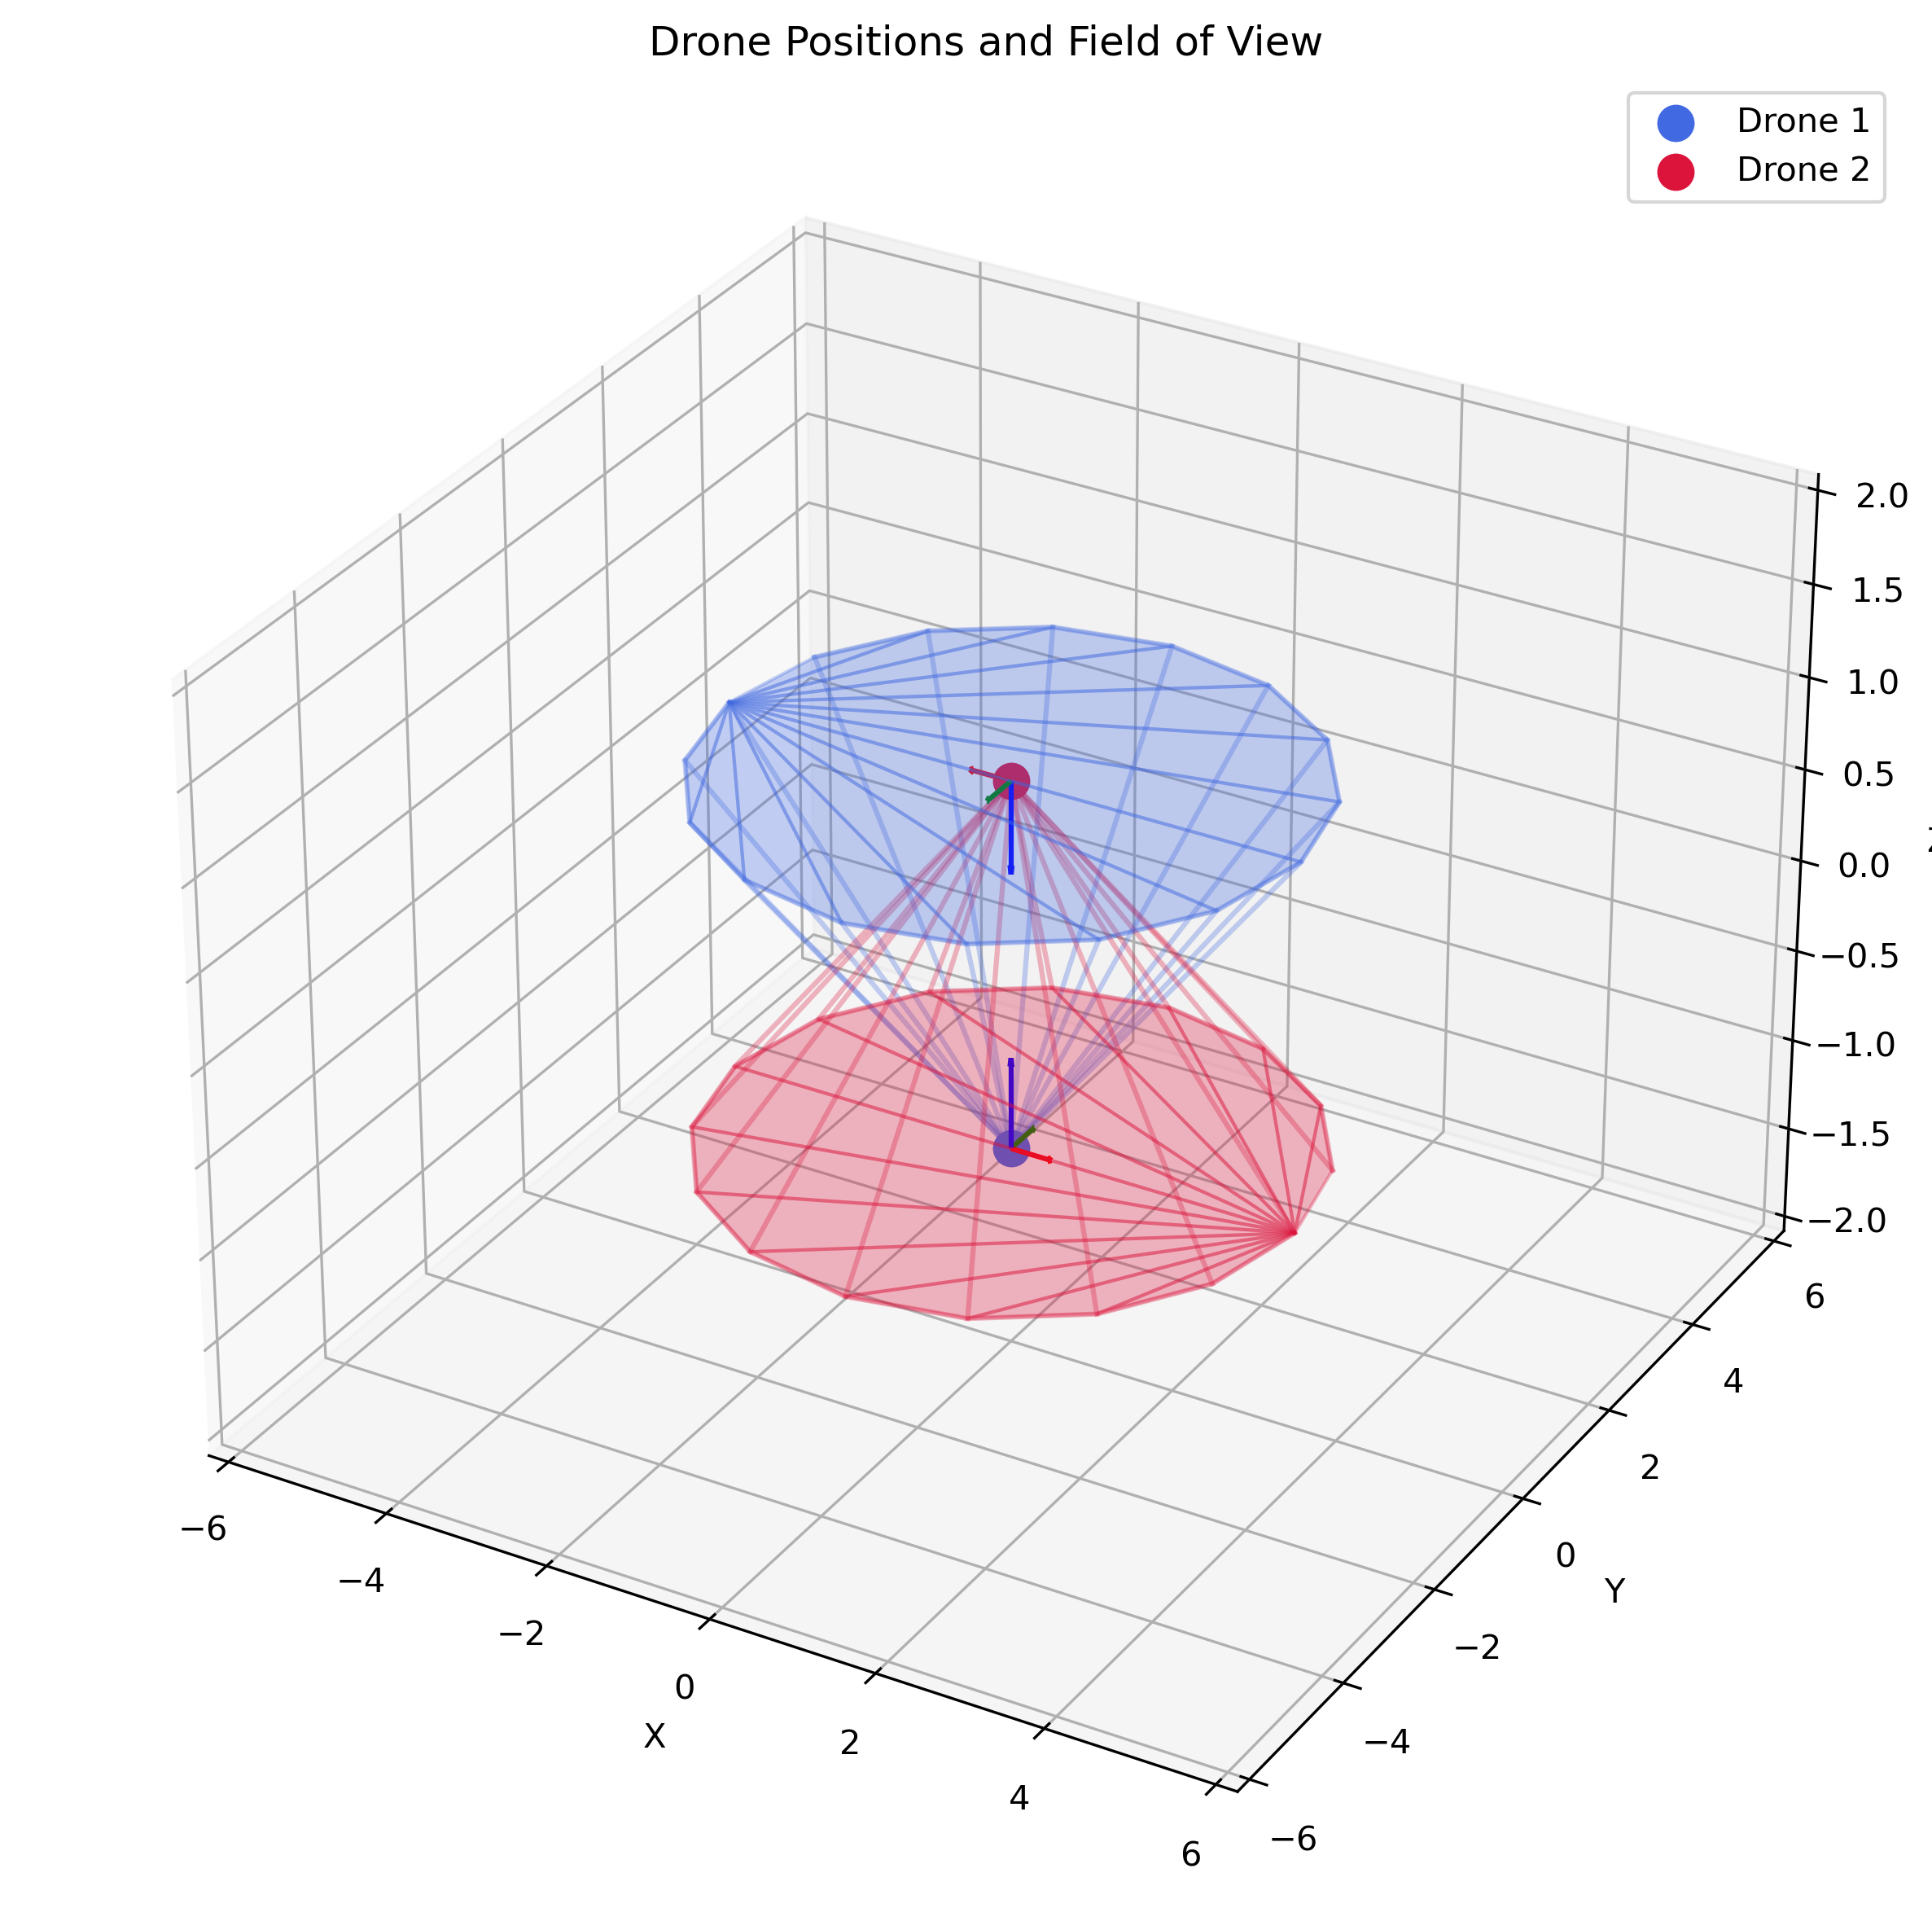
\includegraphics[width=\linewidth]{fig/drone_setup.png}
        \caption{エージェントの設置例}
        \label{fig:drone_setup}
    \end{subfigure}
    \hfill
    \begin{subfigure}[b]{0.45\linewidth}
        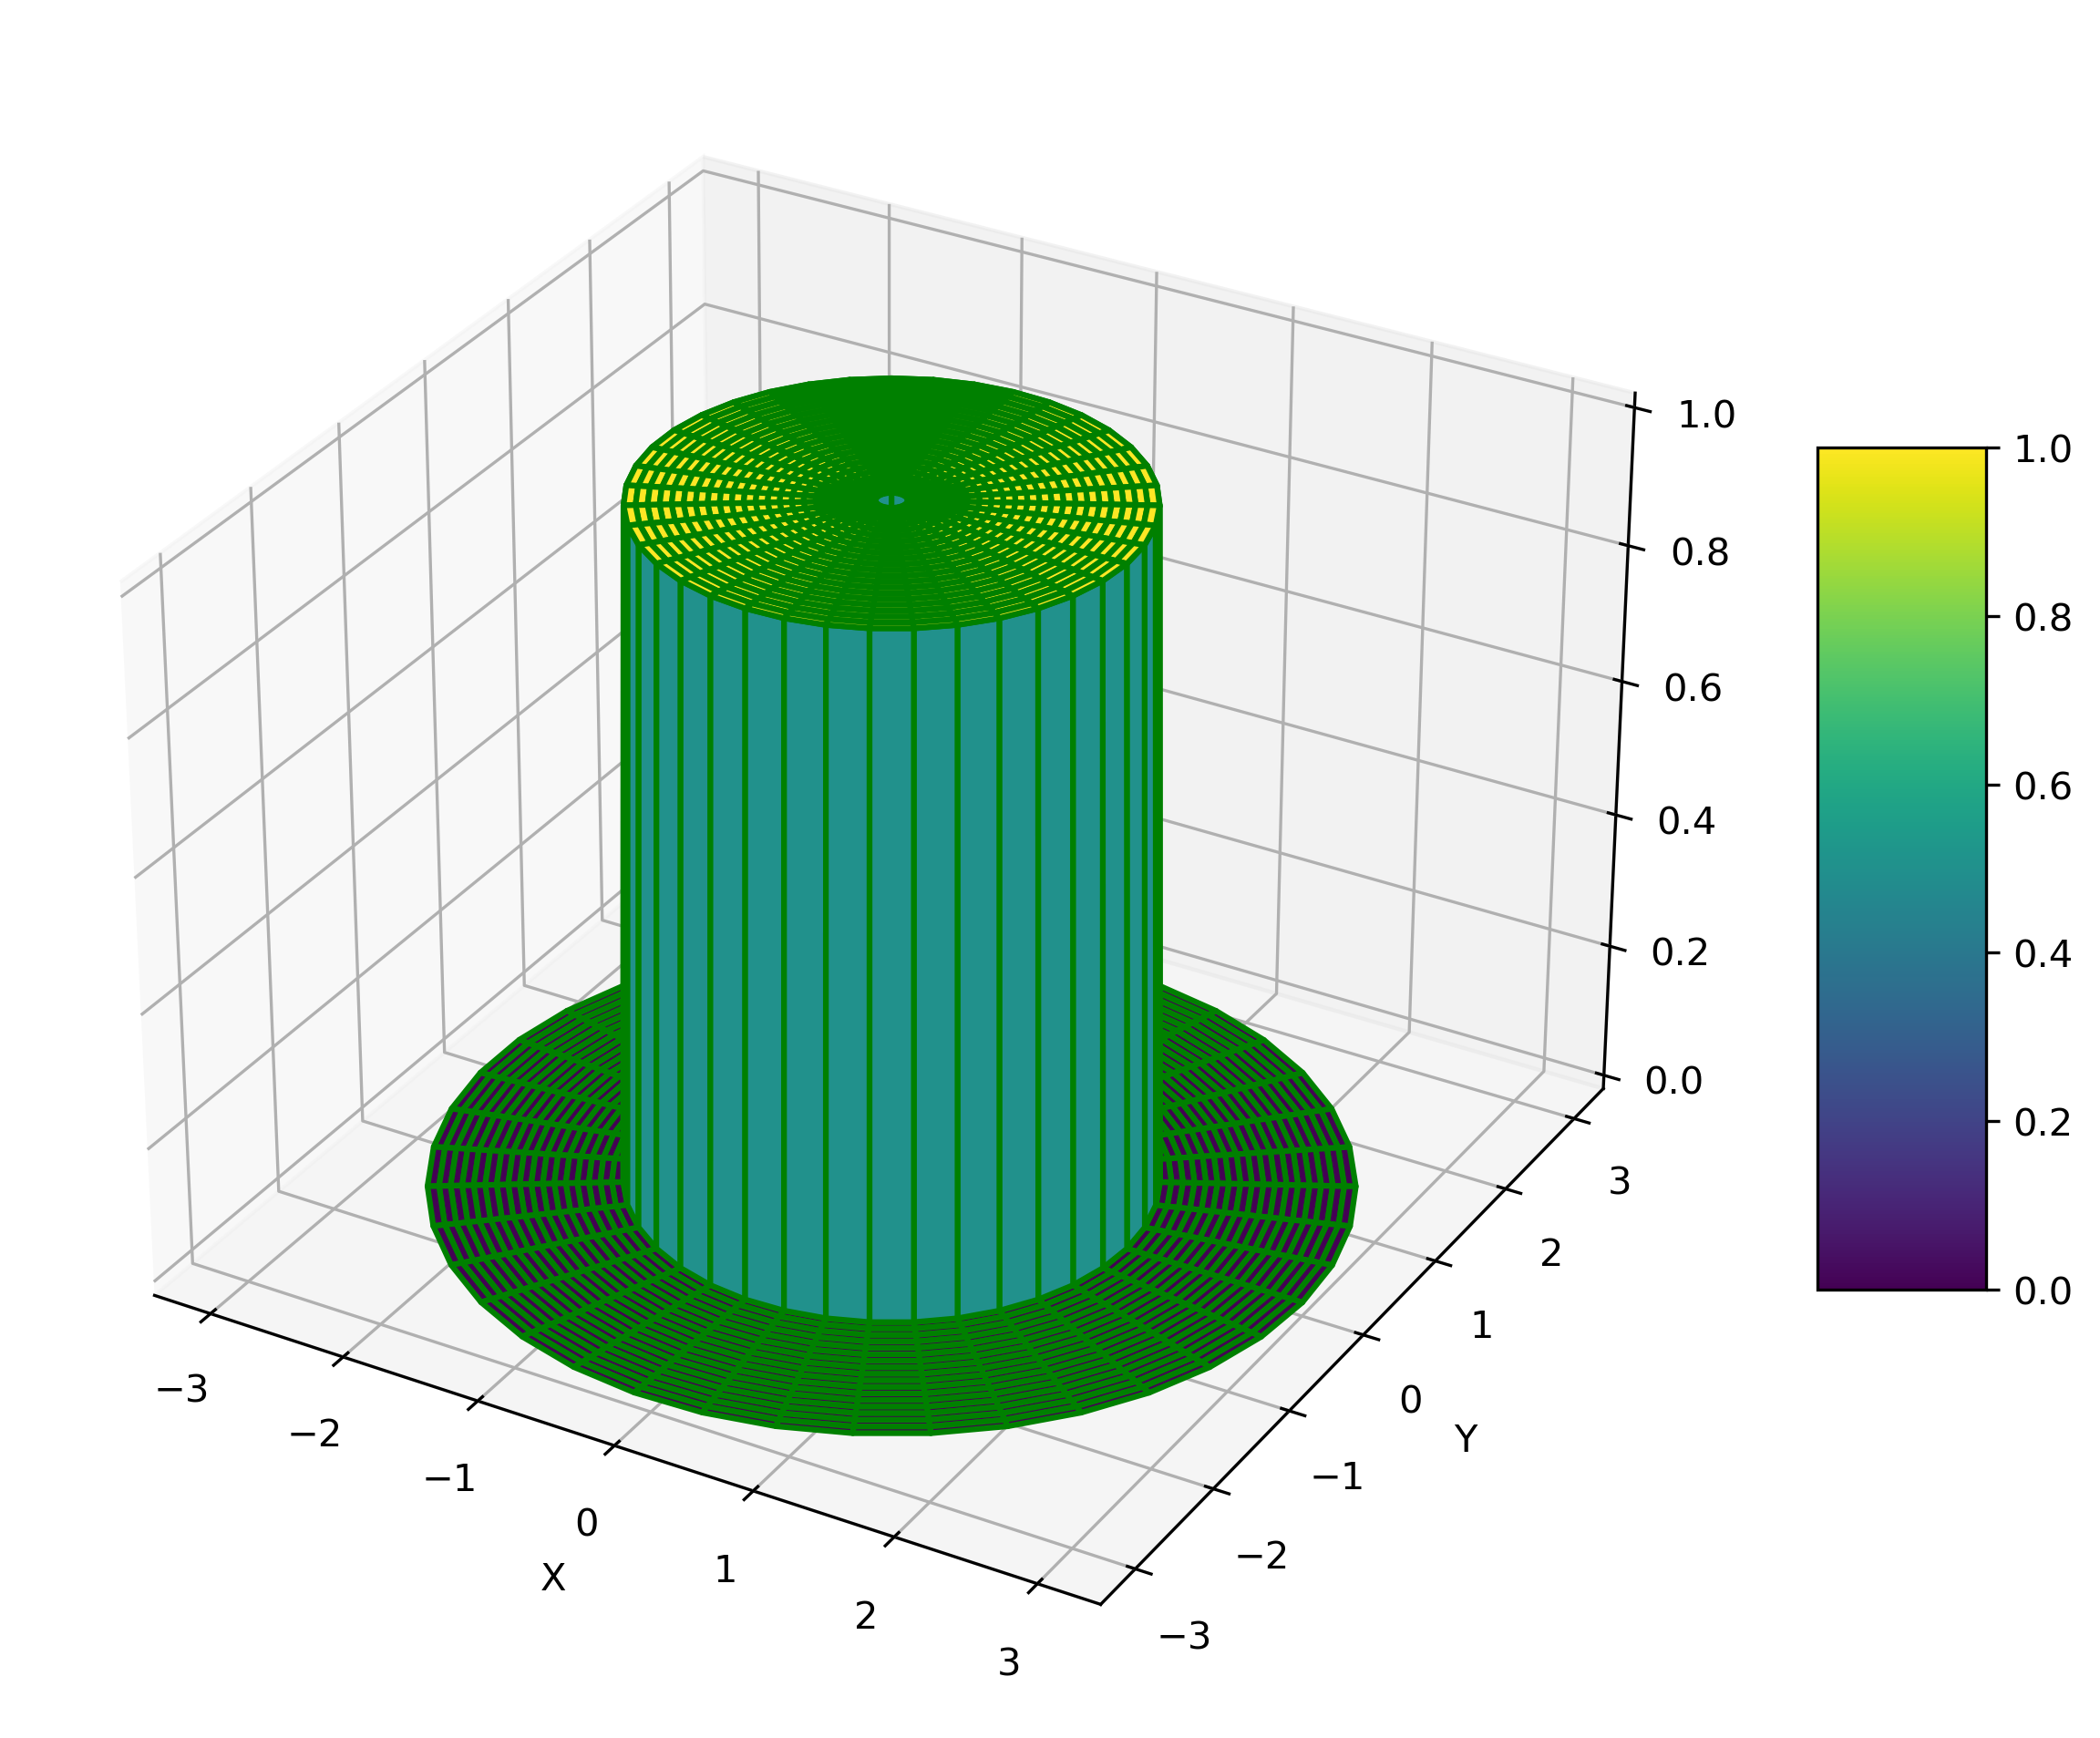
\includegraphics[width=\linewidth]{fig/psi_function_potential.png}
        \caption{$\Psi_{i}^l$関数のポテンシャル\Eqref{eq:psi_function}}
        \label{fig:psi_function_potential}
    \end{subfigure}
    
    \vspace{0.5cm}
    \begin{subfigure}[b]{0.45\linewidth}
        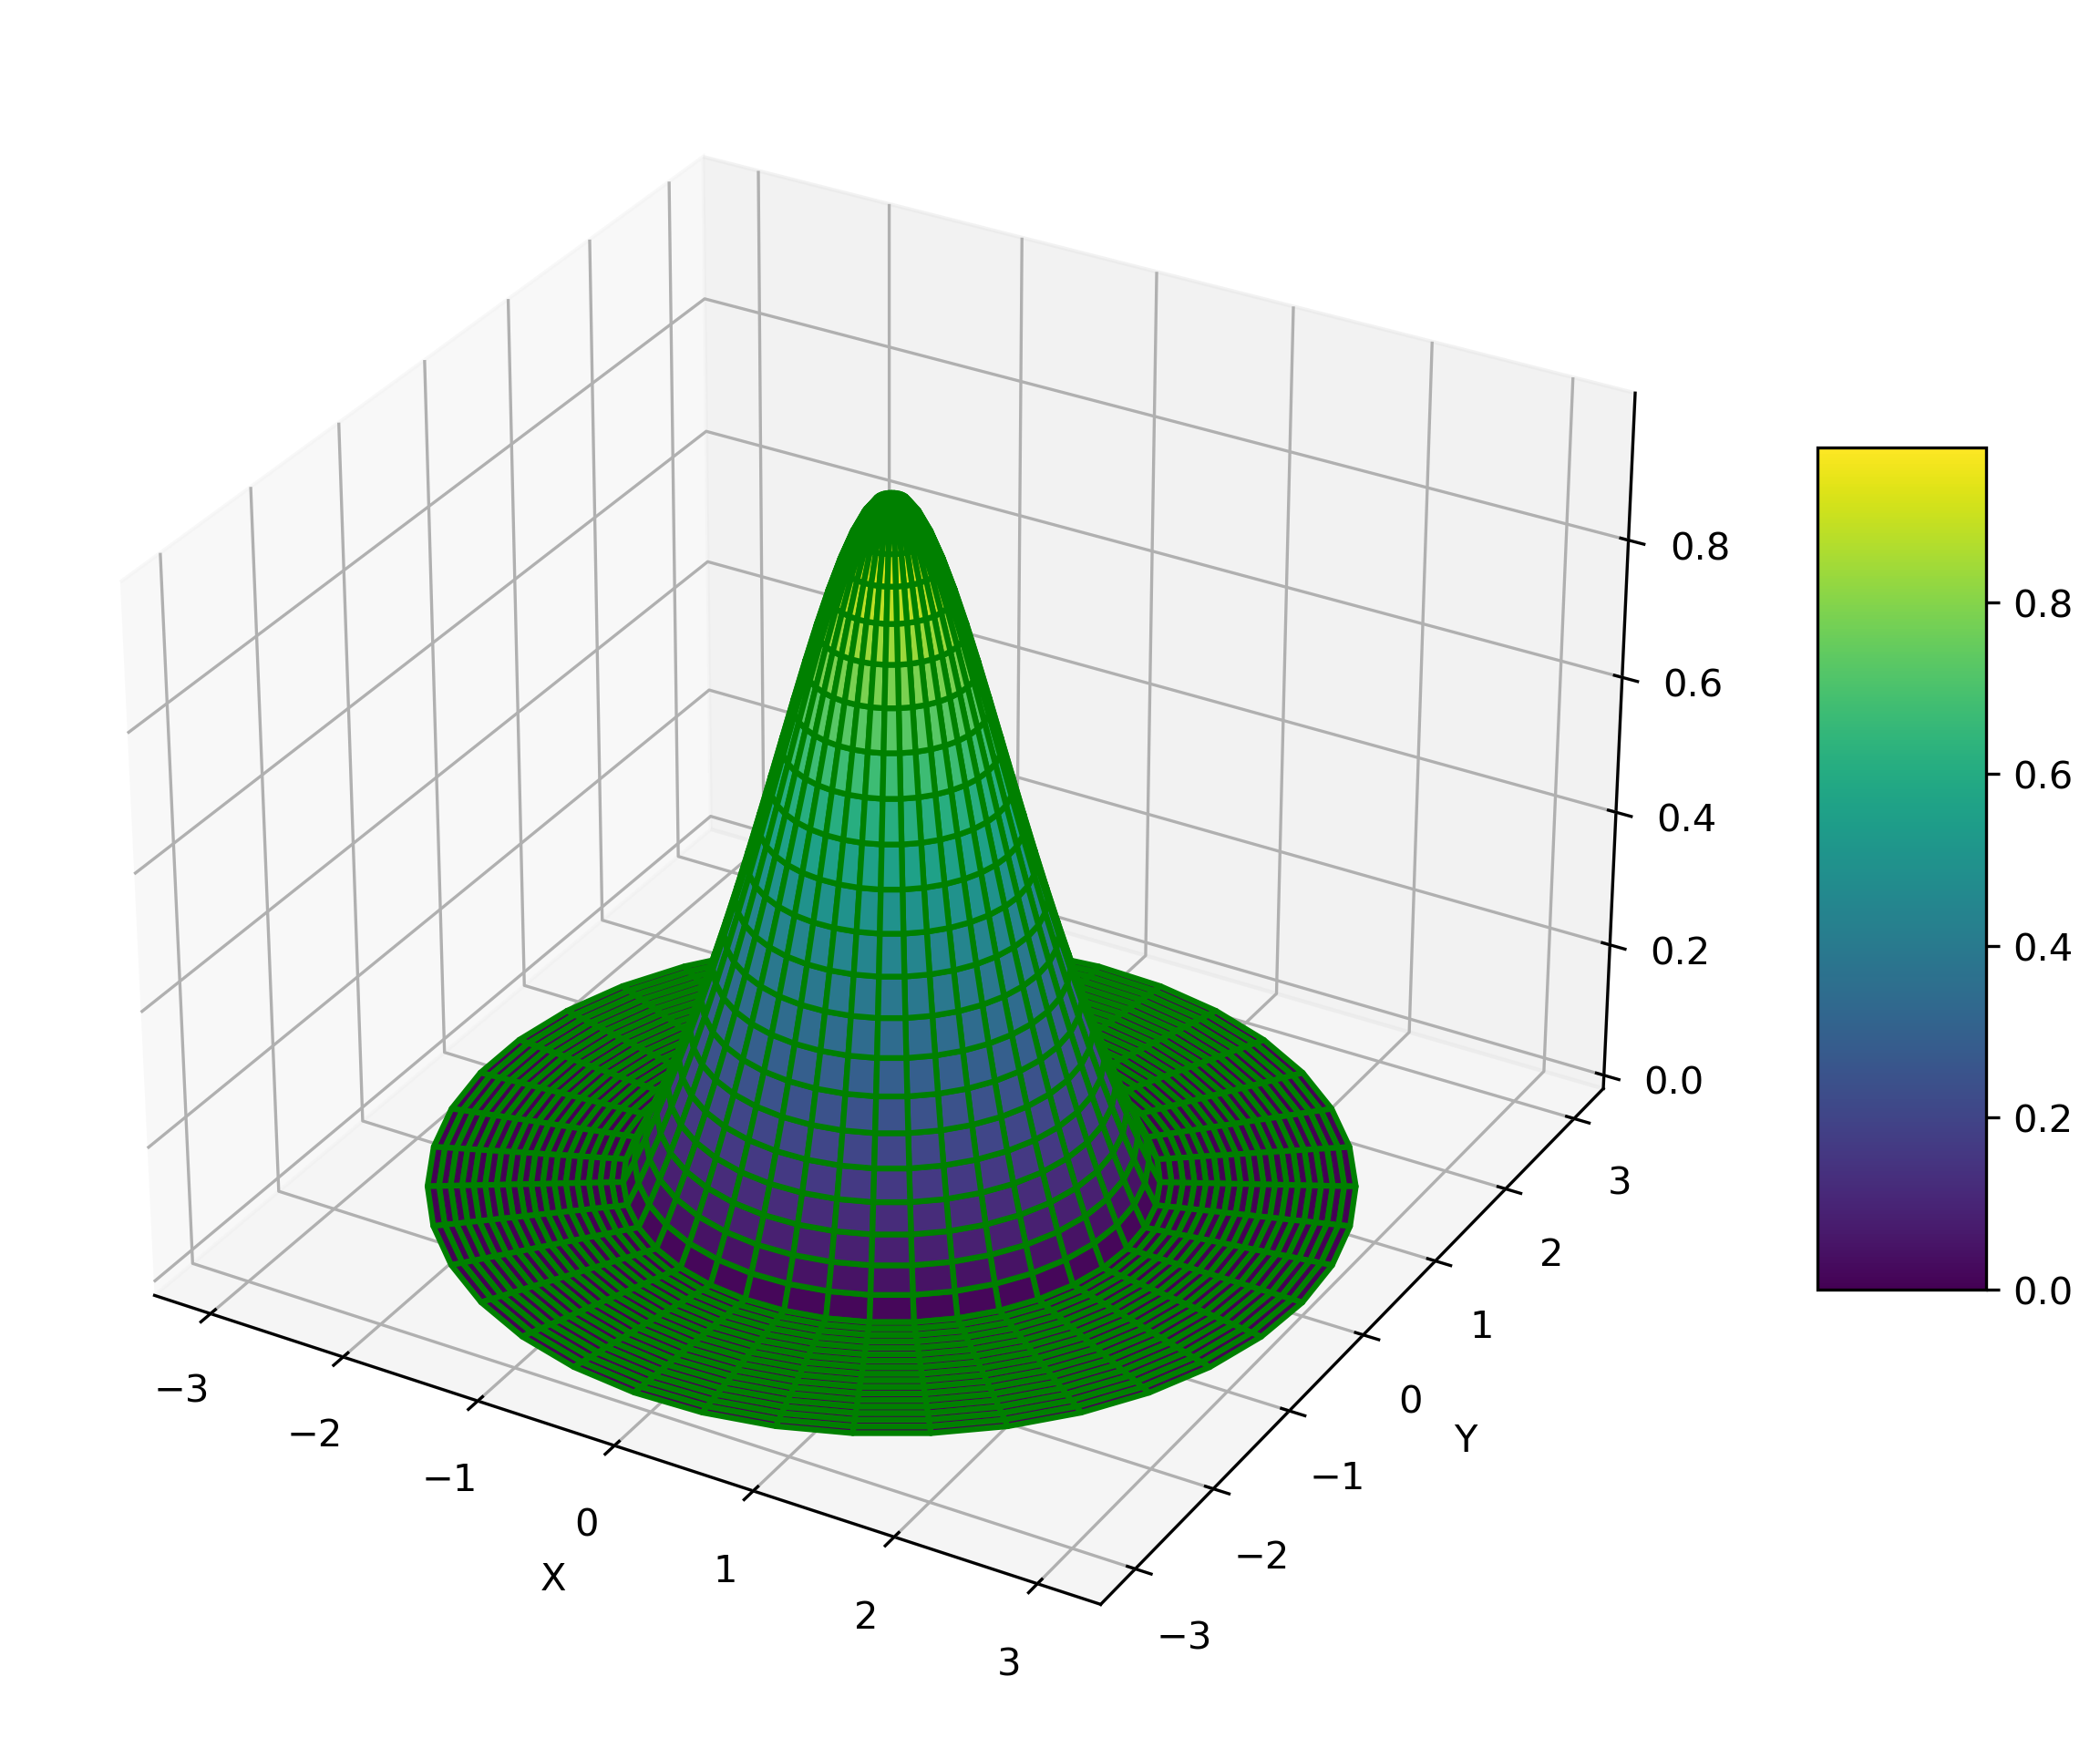
\includegraphics[width=\linewidth]{fig/p_function_potential.png}
        \caption{$P_i^l$関数のポテンシャル\Eqref{eq:new_probability_function}}
        \label{fig:p_function_potential}
    \end{subfigure}
    \hfill
    \begin{subfigure}[b]{0.45\linewidth}
        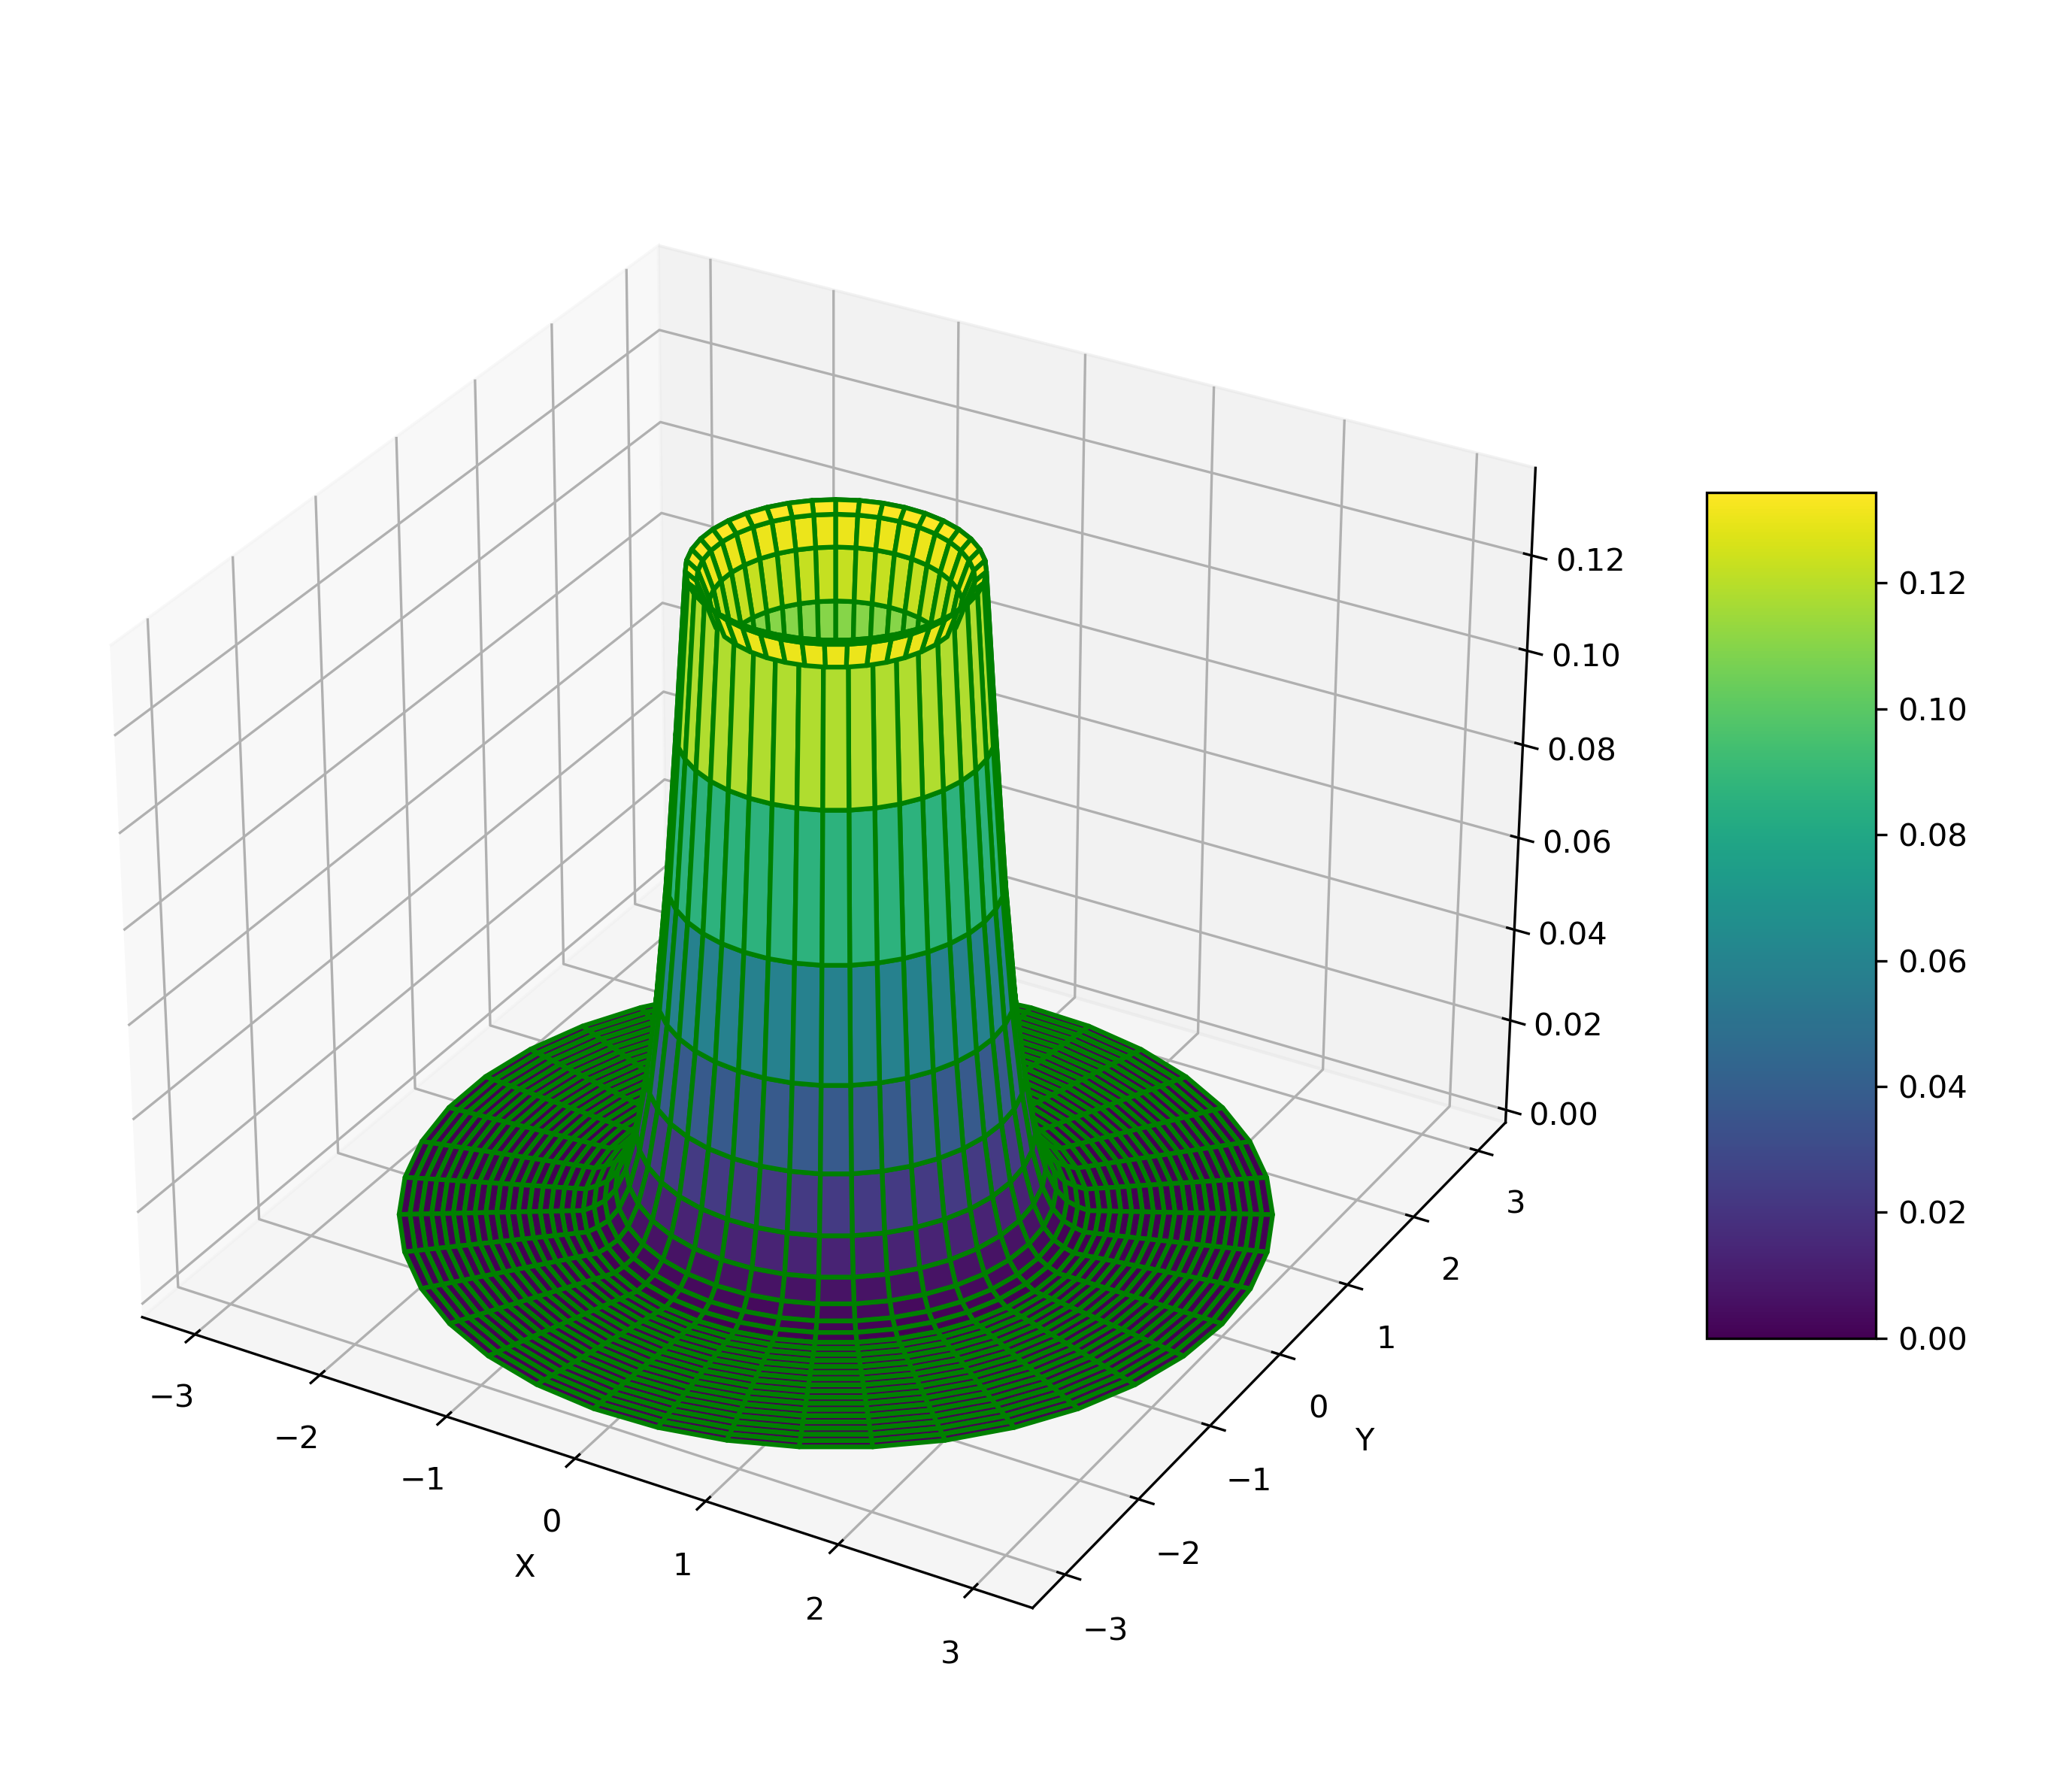
\includegraphics[width=\linewidth]{fig/covariance_function_potential.png}
        \caption{CRLB関数のポテンシャル\Eqref{eq:new_probability_function}}
        \label{fig:covariance_function_potential}
    \end{subfigure}
    \caption{確率関数のポテンシャル}
    \label{fig:potential_comparison}
\end{figure}

また,上記の検討から,\Eqref{eq:new_probability_function}によってCBFを設計する場合,\Figref{fig:CRLB}に示すように,CBFはクラメール・ラオの下限を上から抑える関数として機能することがわかる.クラメール・ラオの下限は最尤推定における最適化限界として働くため,理想的な推定アルゴリズムの元では,視野共有を保証するCBFは自己位置推定を行うためのアクティブパーセプションとして捉えることができる.
\begin{figure}[H]
    \centering
    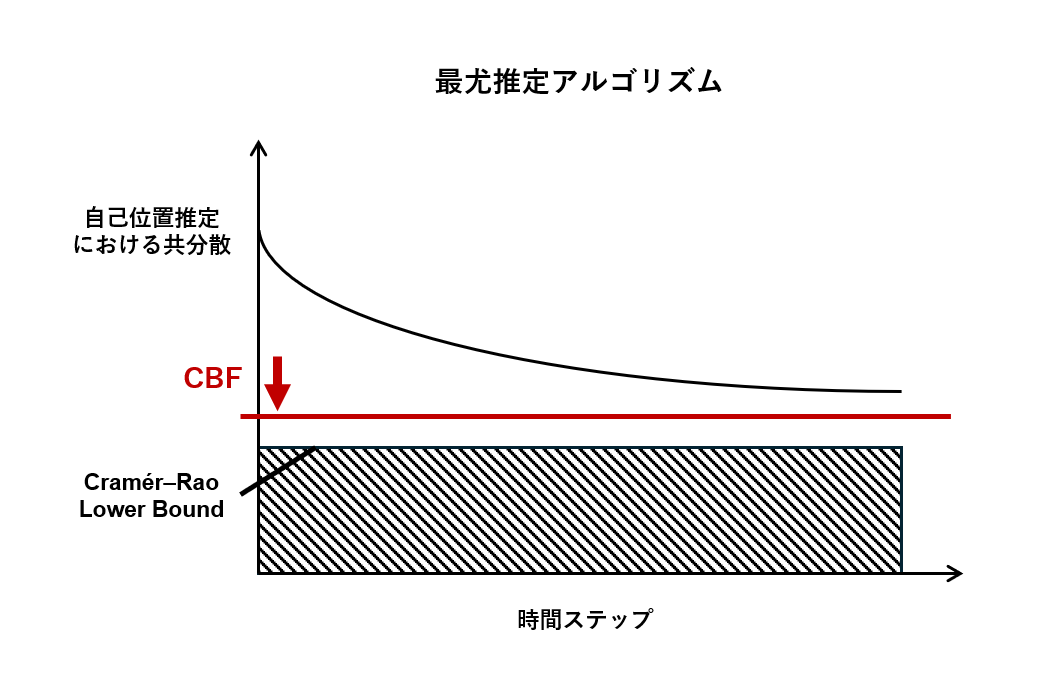
\includegraphics[width=0.7\linewidth]{fig/CRLB.png}
    \caption{クラメール・ラオの下限とCBFの関係}
    \label{fig:CRLB}
\end{figure}

\subsection{確率関数の時間微分と線形化}

確率関数をCBFに適用するには,確率関数の時間微分を制御入力$v_i, v_j$についての線形な関数に変換する必要がある.ここで
\begin{equation}
\begin{aligned}
\dot P_{ij}^l
&= -\frac{\sigma^2}{f^2}\,P_{ij}^l\,\dot T,\\
\dot T
&= \mathrm{tr}\left((M^{-1})^{\cdot}\right)
= -\mathrm{tr}\left(M^{-1}\dot M\,M^{-1}\right).
\end{aligned}
\label{eq:chain_rule}
\end{equation}

ただし$M$は各エージェント $k\in\{i,j\}$ の速度を $w_k=R_k v_k$ とし
\begin{equation}
\begin{aligned}
\dot M
&=\sum_{k\in\{i,j\}}
\frac{\mathrm d}{\mathrm dt}\left(\tfrac{P_{\beta_k}}{d_k^2}\right)\\
&=\sum_{k}
\frac{1}{d_k^2}\dot P_{\beta_k}
-\frac{2\dot d_k}{d_k^3}P_{\beta_k}\\
&=\sum_{k}
\frac{1}{d_k^3}\left[
P_{\beta_k}w_k\beta_k^\top
+\beta_k w_k^\top P_{\beta_k}
+2(\beta_k^\top w_k)P_{\beta_k}
\right].
\end{aligned}
\label{eq:Mdot}
\end{equation}
のように時間微分を計算することができる.

また,トレース演算は以下
\begin{equation}
\begin{aligned}
&\mathrm{tr}\left(M^{-1}\dot M\,M^{-1}\right)\\
&=\sum_{k\in\{i,j\}}
\frac{1}{d_k^3}\left[
\underbrace{\mathrm{tr}(M^{-1}P_{\beta_k}w_k\beta_k^\top M^{-1})}_{t_{k,1}}
+\underbrace{\mathrm{tr}(M^{-1}\beta_k w_k^\top P_{\beta_k}M^{-1})}_{t_{k,2}}
+\underbrace{2(\beta_k^\top w_k)\mathrm{tr}(M^{-1}P_{\beta_k}M^{-1})}_{t_{k,3}}
\right].
\end{aligned}
\label{eq:trace_expand}
\end{equation}
のように分解できる.ただし各項は
$\mathrm{tr}(A\,x\,y^\top\,B)=y^\top B A x$
により
\begin{equation}
\begin{aligned}
t_{k,1}&=w_k^\top P_{\beta_k}M^{-2}\beta_k,\\
t_{k,2}&=w_k^\top P_{\beta_k}M^{-2}\beta_k,\\
t_{k,3}&=2(\beta_k^\top w_k)\,\chi_k,\quad
\chi_k=\mathrm{tr}(M^{-1}P_{\beta_k}M^{-1}).
\end{aligned}
\label{eq:t_terms}
\end{equation}
を得る。よって
\begin{equation}
\begin{aligned}
\mathrm{tr}\left(M^{-1}\dot M\,M^{-1}\right)
&=\sum_{k}
\frac{2}{d_k^3}
w_k^\top\left(P_{\beta_k}M^{-2}\beta_k + \chi_k\beta_k\right).
\end{aligned}
\label{eq:trace_linear}
\end{equation}

上記の変形により,
\eqref{eq:chain_rule}, \eqref{eq:trace_linear} と $w_k=R_k v_k$ を組み合わせ,
\begin{equation}
\begin{aligned}
\dot P_{ij}^l
&=-\frac{\sigma^2}{f^2}P_{ij}^l\left(-\mathrm{tr}(M^{-1}\dot M\,M^{-1})\right)\\
&=\sum_{k\in\{i,j\}}
\lambda_k^\top v_k,
\end{aligned}
\label{eq:Pdot_prel}
\end{equation}
\[
\lambda_k
:=-\frac{2\sigma^2}{f^2}\,
\frac{P_{ij}^l}{d_k^3}\,
R_k^\top\left(P_{\beta_k}M^{-2}\beta_k + \chi_k\beta_k\right).
\]

最終的に
\begin{equation}
\begin{aligned}
\dot P_{ij}^l
= \lambda_i^\top v_i + \lambda_j^\top v_j
\end{aligned}
\label{eq:Pdot_linear}
\end{equation}
が得られる。以上で
$\dot P_{ij}^l$ がエージェント速度 $v_i,v_j$ に対し線形であることを示した。

今後の課題としては,今回シミュレーションを十分に検証できなかった2次系及び非ホロノミック系の結果検証の他,上記で示した自己位置推定における共分散を下限する確率関数の導入を行いたい.
